\documentclass[12pt]{beamer}

\usepackage[brazil]{babel}
\usepackage[utf8]{inputenc}
\usepackage[T1]{fontenc}
\usepackage{animate}
\usepackage{amsbsy}
\usepackage{amsfonts}
\usepackage{amsmath}
\usepackage{amssymb}
\usepackage{amsthm}
\setbeamertemplate{theorems}[numbered] % to number
\usepackage[toc,page,title,titletoc]{appendix}
\usepackage{dsfont}
\usepackage{esvect}
\usepackage[labelfont=bf]{caption}
%\usepackage{subcaption}
\usepackage{float}
\usepackage[Glenn]{fncychap}%Sonny %Conny %Lenny %Glenn %Renje %Bjarne %Bjornstrup
\usepackage{graphicx}
\usepackage{subfig}
\usepackage{indentfirst}%Para indentar os paragrafos automáticamente
\usepackage{lipsum}
\usepackage{longtable}
\usepackage{mathtools}
\usepackage{listings}%Inserir codigo do R no latex
\usepackage{multirow}
\usepackage{multicol}
\usepackage{csquotes}
\usepackage[maxcitenames=2,terseinits=true,natbib=true, style=authoryear, maxbibnames=99]{biblatex}
\addbibresource{../Referencias/Referencias.bib}
\usepackage[figuresright]{rotating}
\usepackage{spalign}
\usepackage{pgfplots}
\pgfplotsset{compat=1.17}
\usepackage{tikz}
\usepackage{fontawesome}
\usepackage{color, colortbl}
\usepackage{url}
\usepackage{cancel}
\usepackage{accents}
\usepackage{bm}
\usepackage{ragged2e}%para justificar o texto dentro de algum ambiente
\definecolor{Gray}{gray}{0.9}
\definecolor{LightCyan}{rgb}{0.88,1,1}


\usepackage[all]{xy}
\usepackage{hyperref,bookmark}
\hypersetup{
  colorlinks=true,
  linkcolor=blue,
  citecolor=red,
  filecolor=blue,
  urlcolor=blue,
}

\usetheme{Madrid}
\usecolortheme[RGB={193,0,0}]{structure}

%\setbeamertemplate{footline}[frame number]
%\setbeamertemplate{footline}[text line]{%
%  \parbox{\linewidth}{\vspace*{-8pt}\hfill\date{}\hfill\insertshortauthor\hfill\insertpagenumber}}
\beamertemplatenavigationsymbolsempty
\renewcommand{\vec}[1]{\mbox{\boldmath$#1$}}
\newtheorem{Teorema}{Teorema}
\newtheorem{Proposicao}{Proposição}
\newtheorem{definicao}{Definição}
\newtheorem{Corolario}{Corolário}
\newtheorem{Demonstracao}{Demonstração}
\newcommand{\bx}{\ensuremath{\bar{x}}}
\newcommand{\Ho}{\ensuremath{H_{0}}}
\newcommand{\Hi}{\ensuremath{H_{1}}}
\newcommand{\at}[2][]{#1|_{#2}}
\newcommand\xuparrow[1][2ex]{%
   \mathrel{\rotatebox{-90}{$\xleftarrow{\rule{#1}{0pt}}$}}
}
\apptocmd{\frame}{}{\justifying}{} % Allow optional arguments after frame.

\makeatletter
\setbeamertemplate{footline}
{
  \leavevmode%
  \hbox{%
  \begin{beamercolorbox}[wd=.3\paperwidth,ht=2.25ex,dp=1ex,center]{author in head/foot}%
    \usebeamerfont{author in head/foot}\mytext
  \end{beamercolorbox}%
  \begin{beamercolorbox}[wd=.3\paperwidth,ht=2.25ex,dp=1ex,center]{title in head/foot}%
    \usebeamerfont{title in head/foot}\mytextt
  \end{beamercolorbox}%
  \begin{beamercolorbox}[wd=.35\paperwidth,ht=2.25ex,dp=1ex,right]{site in head/foot}%
    \usebeamerfont{site in head/foot}\mytexttt\hspace*{2em}
    \insertframenumber{} / \inserttotalframenumber\hspace*{2ex} 
  \end{beamercolorbox}}%
  \vskip0pt%
}
\makeatother

\providecommand{\arcsin}{} \renewcommand{\arcsin}{\hspace{2pt}\textrm{arcsen}}
\providecommand{\sin}{} \renewcommand{\sin}{\hspace{2pt}\textrm{sen}}
\newcommand{\N}{\rm I\!N}
\newcommand{\I}{\rm I\!I}
\newcommand{\R}{\rm I\!R}
\newcommand{\Sim}{\overset{\text{iid}}{\sim}}
\newcommand{\Lim}{{\displaystyle \lim_{n\to\infty}}}
\newcommand{\LimInf}{{\displaystyle \liminf_{n\to\infty}}}
\newcommand{\rightLim}{\xrightarrow[n\rightarrow\infty]{}}
\newcommand{\Sumi}{{\displaystyle \sum_{i=1}^{n}}}
\newcommand{\Int}{{\displaystyle \int_{-\infty}^{+\infty}}}
\newcommand{\ConvD}{\overset{D}{\rightarrow}}
\newcommand{\ConvP}{\overset{P}{\rightarrow}}
\newcommand{\Prodi}{{\displaystyle \prod_{i=1}^{n}}}
\newcommand{\SetaUP}[2]{\underset{\mathclap{\substack{\xuparrow[30pt] \\ #1}}}{#2}}
%\newcommand{\SetaInclinada}[2]{\underset{\mathclap{\substack{\rotatebox{135}{\xuparrow[30pt] \\ #1}}}}{#2}}
\newcommand{\Home}{\begin{tikzpicture}
\node[scale=2] at (3,4) {\text{Para}~\faHome};
\end{tikzpicture}}
\newcommand{\vecX}{\boldsymbol{X}}
\newcommand{\Implica}[1]{\xRightarrow{#1}}
\newcommand{\SeSe}{\iff}
\newcommand{\EscoreA}{\dfrac{\partial}{\partial\theta}\log{f(x,\theta)}}
\newcommand{\EscoreB}{\dfrac{\partial^{2}}{\partial\theta^{2}}\log{f(x,\theta)}}
\newcommand{\cqd}{\text{cqd}~\blacksquare}
\newcommand{\seqX}{$X_{1},\ldots,X_{n}$}
\newcommand{\seqY}{$Y_{1},\ldots,Y_{n}$}
\newcommand{\tend}[1]{\hbox{\oalign{$\bm{#1}$\crcr\hidewidth$\scriptscriptstyle\bm{\sim}$\hidewidth}}}

%\newtheorem{Teorema}{Teorema}
%\newtheorem{Proposicao}{Proposição}
%\newtheorem{Definicao}{Definição}
%\newtheorem{Corolario}{Corolário}
%\newtheorem{Demonstracao}{Demonstração}

\titlegraphic{\hspace*{8cm}\href{https://fsbmat-ufv.github.io/}{
\includegraphics[width=2cm]{figs/mylogo.png}}
}

%Continuar a numeracao em slides diferentes
\newcounter{saveenumi}
\newcommand{\seti}{\setcounter{saveenumi}{\value{enumi}}}
\newcommand{\conti}{\setcounter{enumi}{\value{saveenumi}}}

\resetcounteronoverlays{saveenumi}

% Layout da pagina
\hypersetup{pdfpagelayout=SinglePage}

%Para o \pause funcionar dentro do ambiente align
\makeatletter
\let\save@measuring@true\measuring@true
\def\measuring@true{%
  \save@measuring@true
  \def\beamer@sortzero##1{\beamer@ifnextcharospec{\beamer@sortzeroread{##1}}{}}%
  \def\beamer@sortzeroread##1<##2>{}%
  \def\beamer@finalnospec{}%
}
\makeatother
\setLayoutColor{4} 

\title{Inferência Estatística II}
\author{Prof. Fernando de Souza Bastos\texorpdfstring{\\ fernando.bastos@ufv.br}{}}
\institute{Departamento de Estatística\texorpdfstring{\\ Programa de Pós-Graduação em Estatística Aplicada e Biometria}\texorpdfstring{\\ Universidade Federal de Viçosa}{}\texorpdfstring{\\ Campus UFV - Viçosa}{}}
\date{}
\newcommand\mytext{Aula 10}
\newcommand\mytextt{Fernando de Souza Bastos}
\newcommand\mytexttt{\url{https://est711.github.io/}}


\begin{document}
%\SweaveOpts{concordance=TRUE}

\frame{\titlepage}

% --- INSERIR APÓS \frame{\titlepage} E ANTES DO SUMÁRIO ---

% SLIDE 1/2 — Motivação e perguntas
\begin{frame}{Por que Testes de Hipóteses e Poder importam?}
	\begin{block}{Decidir sob incerteza}
		\justifying
		No mundo real decidimos com dados imperfeitos: aprovar um tratamento, liberar um lote, avaliar uma política. 
		Testes de hipóteses formalizam essa decisão, controlando o \textbf{tamanho} ($\alpha$) e quantificando a capacidade de detectar efeitos reais via \textbf{poder} ($1-\beta$).
	\end{block}
	
	\pause
	\begin{block}{Perguntas-motrizes da aula}
		\begin{itemize}[<+->]
			\item Como controlar erro tipo I e compreender erro tipo II?
			\item O que determina o \textbf{poder} e como aumentá-lo (n, $\sigma$, efeito, $\alpha$)?
			\item Qual a relação entre \textbf{teste bilateral} e \textbf{intervalo de confiança}?
			\item Como interpretar corretamente o \textbf{p-valor}?
		\end{itemize}
	\end{block}
\end{frame}

% SLIDE 2/2 — Objetivos e roteiro
\begin{frame}{O que você levará desta aula}
	\begin{block}{Ao final, você será capaz de}
		\begin{itemize}[<+->]
			\item Derivar/aplicar testes (Z, $t$, proporções, duas amostras) e obter \textbf{valores críticos}.
			\item Traçar e interpretar \textbf{curvas de poder} e seus trade-offs.
			\item Conectar decisão em teste com \textbf{IC}: incluir/excluir $\mu_0$.
			\item Reportar \textbf{p-valor} com ênfase também em \textbf{efeito prático}.
		\end{itemize}
	\end{block}
	
	\pause
	\begin{block}{Roteiro aplicado}
		\justifying
		Exemplos numéricos (média e proporção), cenários uni/bilaterais, comparação de níveis $\alpha$, e visualização interativa do poder (\emph{shiny}) para orientar decisões em pesquisa e indústria.
	\end{block}
\end{frame}
% --- FIM DOS 2 SLIDES INTRODUTÓRIOS ---


\begin{frame}{}
\frametitle{\bf Sumário}
\tableofcontents
\end{frame}

\section{Exemplos}
\subsection{Exemplo 1: Teste Bilateral}
\begin{frame}{Exemplo 1: Teste Bilateral para a Média com Variância Conhecida}
	\begin{block}{}
		\justifying
		Considere $X$ uma variável aleatória com média $\mu$ e variância finita $\sigma^2$. Queremos testar
		\begin{align}\label{t1}
			H_0 : \mu = \mu_0 \quad \text{contra} \quad H_1 : \mu \neq \mu_0
		\end{align}
		onde $\mu_0$ é especificado. Sejam $X_1, \ldots, X_n$ uma amostra aleatória i.i.d. da distribuição de $X$ e denotem a média e a variância amostrais por $\bar{X}$ e $S^2$, respectivamente. Vamos fazer um estudo de sua função poder.
	\end{block}
\end{frame}

\begin{frame}{Regra de decisão (bicaudal)}
	\begin{block}{}
		\justifying
		Para o teste \textbf{bilateral}, rejeitamos $H_0$ quando $\bar{X}$ estiver \emph{muito distante} de $\mu_0$. Assim, para as hipóteses \eqref{t1}, usamos a regra de decisão
		\begin{align}\label{t2}
			\text{Rejeitar } H_0 \text{ em favor de } H_1 \text{ se } \bar{X} \leq h \ \text{ ou } \ \bar{X} \geq k,
		\end{align}
		onde $h<k$ são tais que
		\begin{align}
			\alpha \;=\; P_{H_0} [\bar{X} \leq h \ \text{ ou } \ \bar{X} \geq k]
			= P_{H_0} [\bar{X} \leq h] + P_{H_0} [\bar{X} \geq k].
		\end{align}
	\end{block}
\end{frame}

\begin{frame}{Aproximação assintótica e regiões críticas}
	\begin{block}{}
		\justifying
		Pelo \textbf{TCL} e por \textbf{Slutsky}, sob $H_0$ temos, para $n$ grande,
		\[
		T_n \;=\; \frac{\sqrt{n}\,(\bar X-\mu_0)}{S} \ \xrightarrow{d}\ N(0,1).
		\]
		Logo, uma escolha natural é dividir $\alpha$ igualmente entre as duas caudas da \emph{distribuição assintótica de $T_n$}:
		\begin{align}\label{t3}
			P_{H_0}\!\left[T_n \leq -z_{1-\alpha/2}\right] = \frac{\alpha}{2}
			\quad\text{e}\quad
			P_{H_0}\!\left[T_n \geq z_{1-\alpha/2}\right] = \frac{\alpha}{2}.
		\end{align}
		Isso leva à regra (nível assintótico $\alpha$):
		\begin{align}\label{t4}
			\text{Rejeitar } H_0 \text{ em favor de } H_1 \;\; \text{se} \;\;
			\left|\frac{\bar{X} - \mu_0}{S / \sqrt{n}}\right| \geq z_{1-\alpha/2}.
		\end{align}
	\end{block}
\end{frame}

\begin{frame}{Aproximação assintótica e regiões críticas}
	\begin{block}{}
		\justifying
		Equivalentemente, em termos de $\bar X$,
		\[
		h \approx \mu_0 - z_{1-\alpha/2}\,\frac{S}{\sqrt{n}}
		\quad\text{e}\quad
		k \approx \mu_0 + z_{1-\alpha/2}\,\frac{S}{\sqrt{n}}.
		\]
		\smallskip
		\textit{Observação:} Se $X$ é exatamente Normal, então $T_n \sim t_{(n-1)}$ sob $H_0$ (para qualquer $n$) e podemos usar $t_{1-\alpha/2,(n-1)}$ no lugar de $z_{1-\alpha/2}$.
	\end{block}
\end{frame}


\begin{frame}{}
\begin{block}{}
\justifying
Substituindo $S$ por $\sigma$ e dado que $Z_{1-\alpha/2}=-Z_{\alpha/2}$, segue facilmente que a função poder aproximada é
\begin{align*}\label{t5}
\gamma(\mu) &= P_{\mu}(\bar{X} \leq \mu_0 - |z_{\alpha/2}| \sigma / \sqrt{n}) + P_{\mu}(\bar{X} \geq \mu_0 + |z_{\alpha/2}| \sigma / \sqrt{n})\\
&= \Phi\left(\dfrac{\sqrt{n}(\mu_0 - \mu)}{\sigma} - |z_{\alpha/2}|\right) + 1 - \Phi\left(\dfrac{\sqrt{n}(\mu_0 - \mu)}{\sigma} + |z_{\alpha/2}|\right), 
\end{align*}

em que $\Phi(z)$ é a função de distribuição acumulada de uma variável aleatória normal padrão. Observe que a derivada da função poder é

\begin{align*}
\gamma'(\mu) = \dfrac{\sqrt{n}}{\sigma} \left(\phi\left(\dfrac{\sqrt{n}(\mu_0 - \mu)}{\sigma} + |z_{\alpha/2}|\right) - \phi\left(\dfrac{\sqrt{n}(\mu_0 - \mu)}{\sigma} - |z_{\alpha/2}|\right)\right),
\end{align*}

em que $\phi(z)$ é a função de densidade de probabilidade de uma variável aleatória normal padrão. 
\end{block}
\end{frame}

\begin{frame}{Exercício 4.6.2}
\begin{block}{}
\justifying
Considere $a=\dfrac{\sqrt{n}(\mu_0 - \mu)}{\sigma}$ e notem que,
\begin{itemize}
    \item Se $\mu<\mu_{0},$ então $a>0;$
    \pause
    \item Se $\mu>\mu_{0},$ então $a<0;$
\end{itemize}
\end{block}
\pause 
\begin{block}{}
\justifying
Podemos reescrever então a derivada da função poder como
\begin{align*}
\gamma'(\mu) = \dfrac{\sqrt{n}}{\sigma} \left(\phi\left( |z_{\alpha/2}|+a\right) - \phi\left(|z_{\alpha/2}|-a\right)\right),
\end{align*}
uma vez que $\phi(x)=\phi(-x).$ 
\end{block}
\end{frame}

\begin{frame}{}
\begin{block}{Suponha $\mu<\mu_{0}$}
\justifying
Nesse caso, 
\begin{align*}
    |z_{\alpha/2}|+a>|z_{\alpha/2}|-a&\Rightarrow -\dfrac{(|z_{\alpha/2}|+a)^{2}}{2}<-\dfrac{(|z_{\alpha/2}|-a)^{2}}{2}\\
    &\Rightarrow e^{-\dfrac{(|z_{\alpha/2}|+a)^{2}}{2}} < e^{-\dfrac{(|z_{\alpha/2}|-a)^{2}}{2}}\\
\Rightarrow   \dfrac{\sqrt{n}}{\sigma\sqrt{2\pi}} & \left[e^{-\dfrac{(|z_{\alpha/2}|+a)^{2}}{2}}-e^{-\dfrac{(|z_{\alpha/2}|-a)^{2}}{2}}\right]<0\\
    &\Rightarrow \gamma'(\mu)<0
\end{align*}
\end{block}
\end{frame}


\begin{frame}{}
\begin{block}{Suponha $\mu>\mu_{0}$}
\justifying
Nesse caso, 
\begin{align*}
    |z_{\alpha/2}|+a<|z_{\alpha/2}|-a&\Rightarrow -\dfrac{(|z_{\alpha/2}|+a)^{2}}{2}>-\dfrac{(|z_{\alpha/2}|-a)^{2}}{2}\\
    &\Rightarrow e^{-\dfrac{(|z_{\alpha/2}|+a)^{2}}{2}} > e^{-\dfrac{(|z_{\alpha/2}|-a)^{2}}{2}}\\
    &\Rightarrow \dfrac{\sqrt{n}}{\sigma\sqrt{2\pi}}\left[e^{-\dfrac{(|z_{\alpha/2}|+a)^{2}}{2}}-e^{-\dfrac{(|z_{\alpha/2}|-a)^{2}}{2}}\right]>0\\
    &\Rightarrow \gamma'(\mu)>0
\end{align*}
\end{block}
\end{frame}

\begin{frame}{Conclusões (Teste bilateral, grandes amostras)}
	\begin{block}{}
		\justifying
		\begin{itemize}
			\item \textbf{Pressupostos:} $X_1,\ldots,X_n$ i.i.d., $E[X]=\mu$, $V(X)=\sigma^2<\infty$; $n$ grande.
			\item \textbf{Estatística:} $T_n=\dfrac{\sqrt{n}(\bar X-\mu_0)}{S}\ \overset{H_0}{\xrightarrow{d}}\ N(0,1)$.
			\item \textbf{Regra (nível $\alpha$):} rejeitar $H_0$ se $|T_n|\ge z_{1-\alpha/2}$.\\
			\item \textbf{Função poder:} $\gamma(\mu_0)=\alpha$; $\gamma'(\mu)<0$ se $\mu<\mu_0$ e $\gamma'(\mu)>0$ se $\mu>\mu_0$; \textbf{consistente}: $\gamma(\mu)\to1$ para $\mu\neq\mu_0$ quando $n\to\infty$.
			\item \textbf{Casos especiais:} se $X$ é Normal, usar $t_{n-1}$ no lugar de $z$; se $\sigma$ é conhecido, o teste $Z$ é exato.
			\item \textbf{Prática:} para $n$ pequeno ou caudas pesadas, preferir $t$, transformações, bootstrap ou testes robustos.
		\end{itemize}
	\end{block}
\end{frame}


\subsection{Exemplo 2}
\begin{frame}{Exemplo 2: Teste Bilateral para a Média com Variância Conhecida}
\begin{block}{}
\justifying
Suponha que desejamos testar
\begin{align}
H_0 : \mu = 30,000 \text{ versus } H_1 : \mu \neq 30,000. 
\end{align}

Suponha que $n = 20$ e $\alpha = 0.01$. Então, a regra de rejeição se torna

\begin{align}
\text{Rejeitar } H_0 \text{ em favor de } H_1 \text{ se } \frac{\Bar{X} - 30,000}{\sigma/\sqrt{20}} \geq |z_{\frac{0.01}{2}}|.
\end{align}

A próxima Figura exibe a curva da função poder para este teste quando $\sigma = 5000$. Para comparação, a curva da função poder para o teste com nível $\alpha = 0.05$ também é apresentada. Veja também \href{https://est711.shinyapps.io/FuncaoPoder/}{shiny da função poder!}
\end{block}
\end{frame}


\begin{frame}{}
\begin{block}{}
\justifying
\begin{figure}
    \centering
    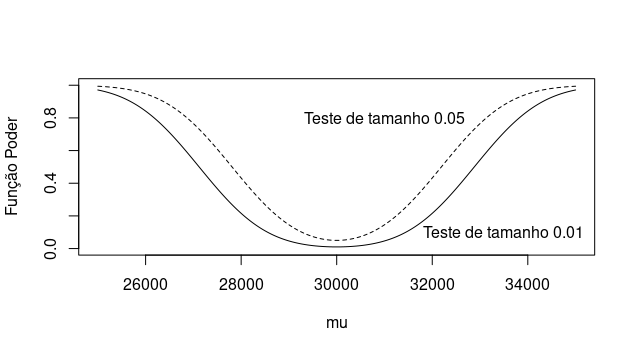
\includegraphics[scale=0.6]{figs/FunctionPower.png}
    \caption{Função Poder para o teste de hipótese do exemplo}
    \label{fig:enter-label}
\end{figure}
\end{block}
\end{frame}

\begin{frame}{Exemplo 3: Teste Bilateral para a Média com Variância Desconhecida}
	\begin{block}{}
		\justifying
		Se $X$ é Normal, então sob $H_0$ temos
		\[
		T=\frac{\bar X-\mu_0}{S/\sqrt{n}} \sim t_{\,n-1}.
		\]
		Logo, o teste bicaudal de tamanho exato $\alpha$ é:
		\[
		\text{Rejeitar } H_0 \text{ se } \left|\frac{\bar X-\mu_0}{S/\sqrt{n}}\right| \ \ge\ t_{1-\alpha/2,\,n-1}.
		\]
		Ele também possui uma curva da função poder em forma de `bacia'' semelhante à Figura anterior, embora não seja tão fácil de mostrar; veja Lehmann (1986).
	\end{block}
\end{frame}


\subsection{Exemplo 4}
\begin{frame}{Exemplo 4: Teste Unilateral para a Média com Variância Conhecida}
\begin{block}{Distribuição Normal:}
\justifying

\begin{itemize}
\item \textbf{Hipótese Nula (H0):} A média de uma população é igual a 100 e \textbf{Hipótese Alternativa (H1):} A média de uma população é maior que 100.
\item $n=30,~\sigma=15$ e $\alpha=0,05$
\item \textbf{Média real sob H1 (Suposição):} 105
\end{itemize}

Para calcular a função poder, usamos a distribuição normal padrão ($Z$) e a fórmula:

\[ \gamma(\mu) = P(Z > Z_{1-\alpha} - \frac{\mu - \mu_0}{\sigma/\sqrt{n}}) \]

em que $Z_{1-\alpha}$ é o valor crítico para o nível de significância $\alpha$.
\end{block}
\end{frame}

\begin{frame}{}
\begin{block}{}
\justifying
Para $\alpha = 0,05$, $Z_{0,95} \approx 1,645.$

Agora, substituindo os valores:
\begin{align*}
    \gamma(105) &= P(Z > 1,645 - \frac{105 - 100}{15/\sqrt{30}})\\
    &= P(Z > 1,645 - 1,826)\\
    &= P(Z > -0,181)
\end{align*}

A probabilidade de $Z$ ser maior que $-0,181$ é aproximadamente $0,5718$. Portanto, o poder do teste é de aproximadamente $0,572$. Logo, com essa amostra, temos cerca de $57{,}2\%$ de chance de rejeitar $H_0$ quando a média verdadeira é $105$. O erro tipo II é $\beta \approx 0{,}428$.

\end{block}
\end{frame}

%\begin{frame}{}
%\begin{block}{Distribuição Binomial}
%\justifying
%\begin{itemize}
%\item \textbf{Hipótese Nula (H0):} A proporção de sucesso em um experimento binomial é de $p_{0}=0,4$.
%\item \textbf{Hipótese Alternativa (H1):} A proporção de sucesso em um experimento binomial é maior que 0,4.
%\item \textbf{Tamanho da amostra:} 100
%\item \textbf{Nível de significância:} 0,01
%\item \textbf{Proporção real sob H1 (Suposição):} 0,55
%\end{itemize}
%
%Para testar uma hipótese sobre uma proporção \( p \) em um experimento binomial, usamos a estatística \( Z \) normalizada sob a hipótese nula:
%\[
%Z = \frac{\hat{p} - p}{\sqrt{\frac{p_0(1 - p_0)}{n}}}
%\]
%onde \( \hat{p} \) é a proporção amostral.
%\end{block}
%\end{frame}
%
%\begin{frame}{}
%\begin{block}{}
%\justifying
%Como \( H_1 \) é unilateral (\( p > 0.4 \)), rejeitamos \( H_0 \) se \( Z \) for maior que o valor crítico \( z_\alpha \). Para \( \alpha = 0.01 \), o valor crítico \( z_\alpha \) é obtido da tabela normal padrão:
%\[
%z_{0.01} = 2.33
%\]
%Isso significa que rejeitamos \( H_0 \) se a estatística \( Z \) for maior que 2.33.
%\end{block}
%\pause
%\begin{block}{}
%	\justifying
%Podemos agora converter o valor crítico de \( Z \) para um valor crítico para a proporção amostral \( \hat{p} \):
%\[
%\hat{p}_{crit} = p_0 + z_{0.01} \times \sqrt{\frac{p_0(1 - p_0)}{n}}
%\]
%Substituindo os valores:
%\[
%\hat{p}_{crit} = 0.4 + 2.33 \times \sqrt{\frac{0.4(1 - 0.4)}{100}}\approx 0.5141
%\]
%Portanto, rejeitamos \( H_0 \) se \( \hat{p} \geq 0.5141 \).
%\end{block}
%\end{frame}
%
%\begin{frame}{}
%	\begin{block}{}
%		\justifying
%A função poder é a probabilidade de rejeitar \( H_0 \) quando a proporção real \( p_1 = 0.55 \). Podemos calcular essa probabilidade usando a mesma estatística \( Z \), mas agora considerando \( p_1 \) como a proporção verdadeira:
%\[
%Z = \frac{\hat{p}_{crit} - p_1}{\sqrt{\frac{p_1(1 - p_1)}{n}}}= \frac{0.5141 - 0.55}{\sqrt{\frac{0.55(1 - 0.55)}{100}}}\approx -0.722
%\]
%Usando a tabela da distribuição normal padrão, encontramos:
%\[
%P(Z > -0.722) = 1 - P(Z \leq -0.722) \approx 1 - 0.2358 = 0.7642
%\]
%Portanto, o \textbf{poder do teste} é aproximadamente \( 0.764 \), ou seja, existe uma probabilidade de cerca de 76,4\% de rejeitar a hipótese nula se a verdadeira proporção for \( 0.55 \).
%		
%	\end{block}
%\end{frame}
%
%\begin{frame}{}
%\begin{block}{}
%\justifying
%\begin{figure}
%    \centering
%    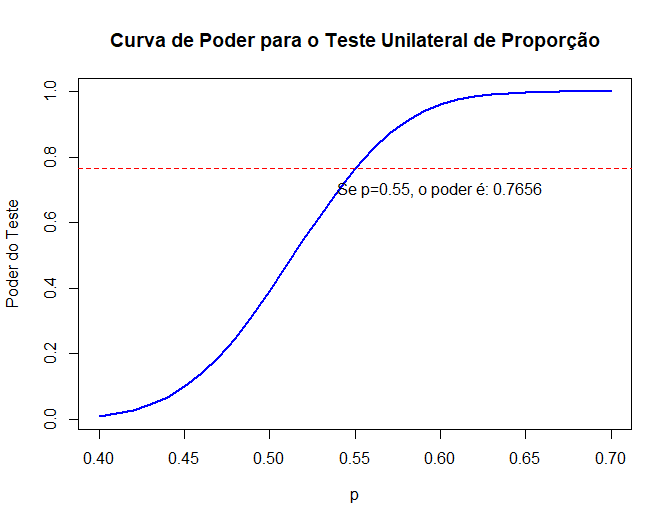
\includegraphics[scale=0.5]{figs/PoderBinomial.png}
%    \caption{Função Poder de um teste unilateral usando a distribuição binomial}
%    \label{fig:enter-label}
%\end{figure}
%\end{block}
%\end{frame}

\subsection{Teste unilateral a direita}
\begin{frame}{Exemplo 5: Teste $Z$ unilateral para a média ($\sigma$ conhecido)}
	\begin{block}{}
		\justifying
		Testar
		\[
		H_0:\ \mu \le \mu_0 \quad \text{vs} \quad H_1:\ \mu > \mu_0,
		\]
		com $\mu_0=100$, $n=36$, $\sigma=12$, $\alpha=0{,}05$. Rejeitamos $H_0$ se
		\[
		Z=\frac{\bar X-\mu_0}{\sigma/\sqrt{n}} > z_{1-\alpha}.
		\]
		Como $z_{1-\alpha}=z_{0{,}95}\approx 1{,}645$, o ponto crítico em termos de $\bar X$ é
		\[
		x_c=\mu_0+z_{1-\alpha}\frac{\sigma}{\sqrt{n}}
		=100+1{,}645\cdot\frac{12}{6}
		=100+3{,}29
		=103{,}29.
		\]
		Logo, rejeite $H_0$ se $\bar X>103{,}29$. Observação: $\alpha=P_{\mu=\mu_0}(\bar X>x_c)$.
	\end{block}
\end{frame}


\begin{frame}{}
%	\begin{block}{Cálculo do Valor Crítico sob $H_{0}$}
%		\justifying
%		\begin{align*}
%			0,05&=P_{\text{Sob}~H_{0}}(\bar{X}>x_{c})=P(Z>\dfrac{(x_{c}-100)\times6}{12})\\
%			&\Rightarrow \dfrac{(x_{c}-100)\times6}{12}=1,645\\
%			&\Rightarrow x_{c}=103,29
%		\end{align*}
%	\end{block}
%	\pause
	\begin{block}{Cálculo do Poder do Teste}
		\justifying
		O poder do teste é a probabilidade de rejeitar $H_0$ quando a verdadeira média $\mu$ é maior que $\mu_0$. Assumindo que a verdadeira média é $\mu = 105:$
		\begin{align*}
			\gamma(\mu=105)&=P_{\mu=105}(\bar{X}>x_{c})=P(\bar{X}>103,29)\\
			&=P(Z>\dfrac{(103,29-105)\times6}{12})=P(Z>-0,855)\\
			&=0,804
		\end{align*}
	\end{block}
\end{frame}

\begin{frame}{}
	\begin{block}{}
		Vejam os gráficos de poder \href{https://est711.shinyapps.io/FuncaoPoder/}{cliquem aqui!}
	\end{block}
\end{frame}

\subsection{Exemplo 6: Teste unilateral a esquerda}
\begin{frame}{Exemplo 6: Teste unilateral para a Média ($\sigma$ conhecido)}
	\begin{block}{}
		\justifying
		Vamos testar a seguinte hipótese nula e alternativa:
		
		\[
		H_0: \mu = \mu_0 = 50 \quad \text{contra} \quad H_1: \mu < 50
		\]
		
		Em que \( \mu_0 = 50 \) é a média sob \( H_0 \), e \( \mu \) é a média populacional desconhecida. Temos uma amostra de tamanho \( n = 36 \), com desvio padrão populacional \( \sigma = 8 \), e o nível de significância \( \alpha = 0.05 \).
		
		
	\end{block}
	\pause
	\begin{block}{}
		\justifying
		Vamos rejeitar $H_0$ se $\bar{X}<x_{c}<50,$ tal que $\alpha=P_{\text{Sob}~H_{0}}(\bar{X}<x_{c})$
		\[
		Z_{\alpha} = -1,645
		\]	
	\end{block}
\end{frame}

\begin{frame}{}
	\begin{block}{Cálculo do Valor Crítico sob $H_{0}$}
		\justifying
		\begin{align*}
			0,05&=P_{\text{Sob}~H_{0}}(\bar{X}<x_{c})=P(Z<\dfrac{(x_{c}-50)\times6}{8})\\
			&\Rightarrow \dfrac{(x_{c}-50)\times6}{8}=-1,645\\
			&\Rightarrow x_{c}=47,81
		\end{align*}
	\end{block}
	\pause
	\begin{block}{Cálculo do Poder do Teste}
		\justifying
		O poder do teste é a probabilidade de rejeitar $H_0$ quando a verdadeira média $\mu$ é menor que $\mu_0$. Vamos assumir que a verdadeira média é $\mu = 47:$
		\begin{align*}
			\gamma(47)&=P_{\mu=47}(\bar{X}<x_{c})=P(\bar{X}<47,81)\\
			&=P(Z<\dfrac{(47,81-47)\times6}{8})=P(Z<0,6075)\\
			&=0,728
		\end{align*}
	\end{block}
\end{frame}

\begin{frame}{}
	\begin{block}{}
		Vejam os gráficos de poder \href{https://est711.shinyapps.io/FuncaoPoder/}{cliquem aqui!}
	\end{block}
\end{frame}

\subsection{Exemplo 7: Teste unilateral para a Proporção Binomial}
\begin{frame}{Exemplo 7: Teste unilateral para a Proporção Binomial}
	\begin{block}{}
		\justifying
		Vamos testar a seguinte hipótese nula e alternativa:
		
		\[
		H_0: p = p_0 = 0,4 \quad \text{contra} \quad H_1: p > 0,4
		\]
		
		O tamanho da amostra é \(n = 100\), o nível de significância é \(\alpha = 0,01\), e assumimos que a proporção real sob \(H_1\) é \(p = 0,55\).
	\end{block}
	\pause
	\begin{block}{}
		\justifying
		Vamos rejeitar $H_0$ se $\bar{p}>p_{c}>0,4,$ tal que $\alpha=P_{\text{Sob}~H_{0}}(\bar{p}>p_{c})$
		\[
		Z_{\alpha} = 2,33
		\]	
	\end{block}
\end{frame}

\begin{frame}{}
	\begin{block}{Cálculo do Valor Crítico sob $H_{0}$}
		\justifying
		\begin{align*}
			0,01&=P_{\text{Sob}~H_{0}}(\bar{p}>p_{c})=P(Z>\dfrac{(p_{c}-0,4)\times10}{\sqrt{0,04\times(1-0,04)}})\\
			&\Rightarrow \dfrac{(p_{c}-0,4)\times10}{\sqrt{0,4\times(1-0,4)}}=2,33\Rightarrow p_{c}=0,5141
		\end{align*}
	\end{block}
	\pause
	\begin{block}{Cálculo do Poder do Teste}
		\justifying
		O poder do teste é a probabilidade de rejeitar $H_0$ quando a verdadeira proporção $p$ é maior que $0,4$. Assumindo que a verdadeira proporção é $p=0,55:$
		\begin{align*}
			\gamma(p=0,55)&=P_{p=0,55}(\bar{p}>p_{c})=P(\bar{p}>0,5141)\\
			&=P(Z>\dfrac{(0,5141-0,55)\times10}{\sqrt{0,55\times(1-0,55)}})=P(Z>-0,722)\\
			&=0,7648
		\end{align*}
	\end{block}
\end{frame}

\begin{frame}{}
	\begin{block}{}
		Vejam os gráficos de poder \href{https://est711.shinyapps.io/FuncaoPoder/}{cliquem aqui!}
	\end{block}
\end{frame}

\subsection{Exemplo 8: Teste Bilateral}
\begin{frame}{Exemplo 8: Teste Bilateral para a Média}
	\begin{block}{}
		\justifying
		Vamos testar:
		\[
		H_0: \mu = \mu_0 = 50 \quad \text{contra} \quad H_1: \mu \neq 50
		\]
		com $n=36$, desvio-padrão populacional conhecido $\sigma=10$ e nível $\alpha=0{,}05$.
	\end{block}
	\pause
	\begin{block}{Regra de decisão e quantis}
		\justifying
		Rejeitar $H_0$ se $\bar X>k$ ou $\bar X<h$, com
		\[
		\frac{\alpha}{2} = P_{H_0}(\bar X>k) = P_{H_0}(\bar X<h),\quad
		z_{1-\alpha/2} = 1{,}96.
		\]
	\end{block}
\end{frame}

\begin{frame}{}
	\begin{block}{Crítico do lado direito ($k$)}
		\justifying
		\begin{align*}
			0{,}025 &= P_{H_0}(\bar X>k) = P\!\left(Z > \frac{k-50}{\sigma/\sqrt{n}}\right)
			= P\!\left(Z > \frac{(k-50)\cdot 6}{10}\right) \\
			&\Rightarrow \frac{(k-50)\cdot 6}{10} = 1{,}96
			\;\Rightarrow\; k = 50 + 1{,}96\cdot \frac{10}{6} = 53{,}27.
		\end{align*}
	\end{block}
	\pause
	\begin{block}{Crítico do lado esquerdo ($h$)}
		\justifying
		\begin{align*}
			0{,}025 &= P_{H_0}(\bar X<h) = P\!\left(Z < \frac{h-50}{\sigma/\sqrt{n}}\right)
			= P\!\left(Z < \frac{(h-50)\cdot 6}{10}\right) \\
			&\Rightarrow \frac{(h-50)\cdot 6}{10} = -1{,}96
			\;\Rightarrow\; h = 50 - 1{,}96\cdot \frac{10}{6} = 46{,}73.
		\end{align*}
	\end{block}
\end{frame}

\begin{frame}{}
	\begin{block}{Função poder (bicaudal)}
		\justifying
		Para $\mu\in\mathbb{R}$,
		\[
		\gamma(\mu) \;=\; P_{\mu}(\bar X>k) \;+\; P_{\mu}(\bar X<h).
		\]
	\end{block}
	\pause
	\begin{block}{Exemplo numérico: $\mu=54$}
		\justifying
		Com $k=53{,}27$, $h=46{,}73$ e $\sigma/\sqrt{n}=10/6\approx 1{,}667$,
		\begin{align*}
		\gamma(54) = P\!\left(Z>\frac{53{,}27-54}{1{,}667}\right) + P\!\left(Z<\frac{46{,}73-54}{1{,}667}\right)\\
		= P(Z>-0{,}438) + P(Z<-4{,}36).
		\end{align*}
		Como $P(Z<-4{,}36)\approx 0$, conclui-se
		\[
		\gamma(54)\approx P(Z>-0{,}438)\approx 0{,}67.
		\]
	\end{block}
\end{frame}


\begin{frame}{}
	\begin{block}{}
		Vejam os gráficos de poder \href{https://est711.shinyapps.io/FuncaoPoder/}{cliquem aqui!}
	\end{block}
\end{frame}

\subsection{Exemplo 9: para Duas Amostras Independentes}
\begin{frame}{Exemplo 9: para Duas Amostras Independentes}
	\vspace{-0.2cm}
	\begin{block}{}
		\justifying
		Considere amostras aleatórias independentes de $N(\mu_1, \sigma^2)$ e $N(\mu_2, \sigma^2)$, respectivamente. Definimos $n = n_1 + n_2$ como o tamanho combinado da amostra e $S_{p}^2$ como o estimador combinado da variância comum, dado por
		\begin{align*}
			S_{c}^2 = \frac{(n_1 - 1)S_1^2 + (n_2 - 1)S_2^2}{n - 2}.
		\end{align*}
		A um nível de significância $\alpha = 0.05$, rejeitamos $H_0 : \mu_1 = \mu_2$ em favor da alternativa unilateral $H_1 : \mu_1 > \mu_2$ se
		\begin{align*}
			T = \frac{\bar{X} - \bar{Y} - 0}{S_c\sqrt{\frac{1}{n_1} + \frac{1}{n_2}}}  \geq t_{0.05, n-2},
		\end{align*}
		pois, sob $H_0$, $T$ segue uma distribuição t com $n - 2$ graus de liberdade.
	\end{block}
\end{frame}

\section{Relação entre Testes de Hipóteses e IC}
\begin{frame}{Relação entre Testes de Hipóteses e IC}
\begin{block}{}
\justifying
Existe uma relação entre testes bilaterais e intervalos de confiança. Considere o teste $t$ bilateral. Aqui, usamos a regra de rejeição com ``se e somente se'' substituindo ``se''. Portanto, em termos de aceitação, temos Aceitar $H_0,$ se, e somente se,

\begin{align*}
\mu_0 - t_{\alpha/2, n-1}S/\sqrt{n} < \Bar{X} < \mu_0 + t_{\alpha/2, n-1}S/\sqrt{n}.
\end{align*}
\end{block}
\pause
\begin{block}{}
Isso pode ser facilmente demonstrado como ``Aceitar $H_0$ se, e somente se'',
\begin{align*}
\mu_0 \in \left(\Bar{X} - t_{\alpha/2, n-1}\frac{S}{\sqrt{n}}, \Bar{X} + t_{\alpha/2, n-1}\frac{S}{\sqrt{n}}\right).
\end{align*}
\end{block}
\end{frame}

\begin{frame}{}
\begin{block}{}
\justifying
Ou seja, aceitamos $H_0$ ao nível de significância $\alpha$ se e somente se $\mu_0$ está no intervalo de confiança de $(1 - \alpha)100\%$ para $\mu$. De forma equivalente, rejeitamos $H_0$ ao nível de significância $\alpha$ se, e somente se, $\mu_0$ não está no intervalo de confiança de $(1 - \alpha)100\%$ para $\mu$. Isso é válido para todos os testes de hipóteses bilaterais.
\end{block}
\end{frame}

\subsection{Exemplo 10 - Distribuição Binomial}
\begin{frame}{Exemplo 10 - Distribuição Binomial}
\begin{block}{}
\justifying
Suponha que $X$ segue uma distribuição binomial com parâmetros $1$ e $p$. Considere o teste de hipótese $H_0 : p = p_0$ contra $H_1 : p < p_0$. Seja $X_1, \ldots, X_n$ uma amostra aleatória da distribuição de $X$, e seja $\hat{p} = \frac{X}{n}$. Para testar $H_0$ versus $H_1$, utilizamos uma das seguintes estatísticas:

\begin{align*}
Z_1 = \frac{\hat{p} - p_0}{\sqrt{p_0(1 - p_0)/n}} \leq c~\text{ou}~Z_2 = \frac{\hat{p}-p_0}{\sqrt{\hat{p}(1 - \hat{p})/n}} \leq c.
\end{align*}

Se o tamanho da amostra $n$ for grande, tanto $Z_1$ quanto $Z_2$ têm distribuições normais aproximadas, desde que $H_0 : p = p_0$ seja verdadeira. Portanto, se $c$ for definido como $-1.645$, o nível de significância aproximado é $\alpha = 0.05$. Ambos os métodos fornecem resultados numéricos semelhantes.
\end{block}
\end{frame}


\begin{frame}{}
\begin{block}{}
\justifying
Com uma hipótese alternativa bilateral, $Z_2$ fornece uma melhor relação com o intervalo de confiança para $p$. Ou seja, $|Z_2| < z_{\alpha/2}$ é equivalente a $p_0$ estar no intervalo

\begin{align*}
\left(\hat{p} - z_{\alpha/2}\sqrt{\frac{\hat{p}(1 - \hat{p})}{n}}, \hat{p} + z_{\alpha/2}\sqrt{\frac{\hat{p}(1 - \hat{p})}{n}}\right),
\end{align*}

que é o intervalo que fornece um intervalo de confiança aproximado de $(1 - \alpha)100\%$ para $p$, conforme discutido na aula de Intervalos de Confiança. Vejam os gráficos de poder \href{https://est711.shinyapps.io/FuncaoPoder/}{cliquem aqui!}
\end{block}
\end{frame}



%\begin{frame}{}
%\begin{block}{}
%\justifying
%No entanto, um nível de significância de $\alpha = 0.05$ pode ser alcançado da seguinte maneira. Seja $W$ uma variável aleatória com distribuição de Bernoulli com probabilidade de sucesso igual a
%
%\begin{align*}
%P(W = 1) = \frac{\alpha-0.019}{0.08-0.019}=\frac{0.050 - 0.019}{0.080 - 0.019} = \frac{31}{61}.
%\end{align*}
%
%Suponha que $W$ seja selecionado independentemente da amostra. Considere a regra de rejeição: rejeitar $H_0$ se $\sum_{i=1}^{10} X_i \geq 4$ ou se $\sum_{i=1}^{10} X_i = 3$ e $W = 1$. O nível de significância dessa regra é
%{\small 
%\begin{align*}
%P_{H_0}(Y \geq 4) + P_{H_0}(\{Y = 3\} \cap \{W = 1\})&= P_{H_0}(Y \geq 4)\\ + P_{H_0}(Y = 3)P(W = 1)\\ &= 0.019 + 0.061 \times \frac{31}{61}\\ &= 0.05.
%\end{align*}}
%\end{block}
%\end{frame}
%
%\begin{frame}{}
%\begin{block}{}
%\justifying
%Portanto, a regra de decisão tem exatamente um nível de 0.05. O processo de realizar o experimento auxiliar para decidir se rejeita ou não quando $Y = 3$ é às vezes referido como um teste randomizado.
%\end{block}
%\end{frame}

%\section{Nível de Significância Observado (p-valor)}

\subsection{Exemplo 1 - Distribuição Poisson}
\begin{frame}{Exemplo - Distribuição Poisson}
	\begin{block}{}
		\justifying
		Seja $X_1, X_2, \ldots, X_{10}$ uma amostra aleatória de tamanho $n = 10$ de uma distribuição de Poisson com média $\theta$. A região crítica para testar $H_0 : \theta = 0.1$ contra $H_1 : \theta > 0.1$ é dada por $Y = {\displaystyle \sum_{i=1}^{10}} X_i \geq 3$. A estatística $Y$ segue uma distribuição de Poisson com média $10\theta$. Portanto, com $\theta = 0.1$, a média de $Y$ é 1, o nível de significância do teste é
		
		\begin{align*}
			P(Y \geq 3) = 1 - P(Y \leq 2) = 1 - 0.920 = 0.080.
		\end{align*}
	\end{block}
\end{frame}

\begin{frame}{}
	\begin{block}{}
		\justifying
		Por outro lado, se a região crítica definida por $\sum_{i=1}^{10} X_i \geq 4$ for usada, o nível de significância é
		
		\begin{align*}
			\alpha = P(Y \geq 4) = 1 - P(Y \leq 3) = 1 - 0.981 = 0.019.
		\end{align*}
		
		Por exemplo, se um nível de significância de aproximadamente $\alpha = 0.05$ for desejado, a maioria dos estatísticos usaria um desses testes, ou seja, eles ajustariam o nível de significância para o teste mais conveniente. 
	\end{block}
\end{frame}

\begin{frame}{Nível de Significância Observado (p-valor)}
\begin{block}{}
\justifying
Muitos estatísticos não gostam de testes randomizados na prática. %pois o uso deles implica que dois estatísticos podem fazer as mesmas suposições, observar os mesmos dados, aplicar o mesmo teste e, no entanto, tomar decisões diferentes (Pois a decisão final pode depender de um sorteio). Portanto, eles costumam ajustar seu nível de significância para evitar a aleatoriedade. 
Na verdade, muitos estatísticos relatam o que são comumente chamados de níveis de significância observados ou valores-p (para valores de probabilidade). Um exemplo geral é suficiente para explicar os níveis de significância observados.  
\end{block}
\end{frame}

\begin{frame}{}
\begin{block}{}
\justifying
Seja $X_1, \ldots, X_n$ uma amostra aleatória de uma distribuição $N(\mu, \sigma^2)$, em que tanto $\mu$ quanto $\sigma^2$ são desconhecidos. Considere, primeiro, as hipóteses unilaterais $H_0 : \mu = \mu_0$ versus $H_1 : \mu > \mu_0$, em que $\mu_0$ é especificado. Escreva a regra de rejeição como

\begin{align}
\text{Rejeitar } H_0 \text{ em favor de } H_1, \text{ se } \Bar{X} \geq k, 
\end{align}
em que $\Bar{X}$ é a média da amostra.
\end{block}
\pause
\begin{block}{}
\justifying
Anteriormente, especificamos um nível e, em seguida, resolvemos para $k$. Na prática, no entanto, o nível não é especificado. Em vez disso, uma vez que a amostra é observada, o valor realizado $\Bar{x}$ de $\Bar{X}$ é calculado e fazemos a pergunta: O valor $\Bar{x}$ é suficientemente grande para rejeitar $H_0$ em favor de $H_1$? 
\end{block}
\end{frame}

\begin{frame}{}
\begin{block}{}
\justifying
Para responder a isso, calculamos o valor-p, que é a probabilidade,

\begin{align*}
\text{valor-p} = P_{\text{Sob}~H_0}( \Bar{X} \geq \Bar{x}).
\end{align*}

Observe que este é um ``nível de significância'' baseado nos dados, e chamamos isso de nível de significância observado ou valor-p. 
\end{block}
\end{frame}

\begin{frame}{}
\begin{block}{}
\justifying
A hipótese $H_0$ é rejeitada em todos os níveis maiores ou iguais ao valor-p. Por exemplo, se o valor-p for $0,048$ e o nível nominal $\alpha$ for $0,05$, então $H_0$ será rejeitada; no entanto, se o nível nominal $\alpha$ for $0,01$, então $H_0$ não será rejeitada. Em resumo, o experimentador define as hipóteses; o estatístico seleciona a estatística de teste e a regra de rejeição; os dados são observados e o estatístico relata o valor-p para o experimentador; e o experimentador decide se o valor-p é suficientemente pequeno para justificar a rejeição de $H_0$ em favor de $H_1$. O próximo exemplo fornece uma ilustração numérica.
\end{block}
\end{frame}

\subsection{Exemplo 2 (Valor - p)}
\begin{frame}{Exemplo (Valor - p)}
\begin{block}{}
\justifying
Considere os dados de Darwin do Exemplo 4.5.5 do livro do Hogg (Edição 8). Os dados são um design emparelhado sobre as alturas de plantas de Zea mays cruzadas e autofertilizadas. Em cada um dos 15 vasos, uma planta cruzada e uma autofertilizada foram cultivadas. Os dados de interesse são as 15 diferenças emparelhadas, (cruzada - autofertilizada). Como no Exemplo, deixe $X_i$ denotar a diferença emparelhada para o i-ésimo vaso. Deixe $\mu$ ser a verdadeira diferença média. As hipóteses de interesse são $H_0 : \mu = 0$ versus $H_1 : \mu > 0$. A regra de rejeição padronizada é

\begin{align}
\text{Rejeitar } H_0 \text{ em favor de } H_1 \text{ se } T \geq k,
\end{align}

em que $T = \frac{\Bar{X}}{S/\sqrt{15}}$, $\Bar{X}$ e $S$ são, respectivamente, a média amostral e o desvio padrão das diferenças. 
\end{block}
\end{frame}

\begin{frame}{}
\begin{block}{}
\justifying
A hipótese alternativa afirma que, em média, as plantas cruzadas são mais altas do que as plantas autofertilizadas. Do Exemplo 4.5.5, a estatística do teste t tem o valor 2,15. Deixando $t(14)$ denotar uma variável aleatória com a distribuição t com 14 graus de liberdade e usando R, o valor-p para o experimento é

\begin{align*}
P[t(14) > 2.15] = 1 - pt(2.15, 14) = 1 - 0.9752 = 0.0248. 
\end{align*}

Na prática, com esse valor-p, $H_0$ seria rejeitada em todos os níveis maiores ou iguais a 0,0248.

Suponha que as hipóteses sejam $H_0 : \mu = \mu_0$ versus $H_1 : \mu < \mu_0$. Obviamente, o valor-p observado neste caso é

\begin{align*}
\text{valor-p} = P_{\text{Sob}~H_0}( \Bar{X} \geq \Bar{x}).
\end{align*}
\end{block}
\end{frame}

\begin{frame}{}
\begin{block}{}
\justifying
Para a hipótese bilateral $H_0 : \mu = \mu_0$ versus $H_1 : \mu \neq \mu_0$, nossa regra de rejeição ``não especificada'' é

\begin{align}
\text{Rejeitar } H_0 \text{ em favor de } H_1 \text{ se } \Bar{X} \leq l \text{ ou } \Bar{X} \geq k.
\end{align}

Para o valor-p, calculamos cada um dos valores-p de um lado, pegamos o menor valor-p e o dobramos. Como ilustração, no exemplo de Darwin, suponha que as hipóteses sejam $H_0 : \mu = 0$ versus $H_1 : \mu \neq 0$. Então, o valor-p é $2 \times (0,0248) = 0,0496$. 
\nocite{hogg}
\end{block}
\end{frame}

%\begin{frame}{}
%\begin{block}{}
%\justifying
%Como nota final sobre valores-p para hipóteses bilaterais, suponha que a estatística de teste possa ser expressa em termos de uma estatística de teste t. Nesse caso, o valor-p pode ser encontrado de forma equivalente da seguinte maneira. Se $d$ for o valor realizado da estatística de teste t, então o valor-p é
%
%\begin{align}
%\text{valor-p} = P(H_0 [|t| \geq |d|]), 
%\end{align}
%
%em que, sob $H_0$, $t$ tem uma distribuição $t$ com $n - 1$ graus de liberdade.
%\end{block}
%\pause
%\begin{block}{}
%\justifying
%Nessa discussão sobre valores-p, lembre-se de que a boa ciência dita que as hipóteses devem ser conhecidas antes que os dados sejam coletados.
%\end{block}
%\end{frame}


%\begin{frame}{}
%\begin{block}{Explicação Detalhada:}
%\justifying
%O valor-p é uma medida estatística que ajuda a avaliar a força das evidências contra uma hipótese nula em um teste de hipóteses. Ele é calculado com base nos dados observados e na distribuição da estatística de teste sob a suposição de que a hipótese nula é verdadeira. 
%\end{block}
%\pause
%\begin{block}{}
%\justifying
%Ele não é estritamente uma probabilidade no sentido tradicional. Embora seja comumente interpretado como uma probabilidade, é uma medida de evidência estatística em vez de uma probabilidade direta de um evento.
%\end{block}
%\pause
%\begin{block}{}
%\justifying
%O valor-p é, portanto, uma medida de quão consistentes os dados observados são com a hipótese nula. É a probabilidade de obter resultados tão extremos quanto os observados, assumindo que a hipótese nula seja verdadeira.
%\end{block}
%\end{frame}

%\begin{frame}{}
%\begin{block}{Aqui estão as etapas para entender o valor-p:}
%
%\begin{itemize}
%\justifying
%\item Formulação das Hipóteses:
%
%A primeira etapa é estabelecer duas hipóteses: a hipótese nula ($H_0$) e a hipótese alternativa ($H_1$). \pause
%
%\item Coleta de Dados:
%
%Em seguida, você coleta dados relevantes para o teste de hipóteses.\pause
%
%\item Cálculo da Estatística de Teste:
%
%Você calcula uma estatística de teste com base nos dados. A escolha da estatística depende do tipo de teste e da pergunta de pesquisa.
%\end{itemize}
%\end{block}
%\end{frame}

%\begin{frame}{}
%\begin{block}{}
%\justifying
%\begin{itemize}
%\justifying
%\item Determinação do Valor-p 
%
%Com a estatística de teste em mãos, você calcula o Valor-p. Esse cálculo envolve a probabilidade de obter uma estatística de teste tão extrema quanto a observada, supondo que a hipótese nula seja verdadeira. Essa probabilidade é chamada de Valor-p.\pause
%
%\item Interpretação do Valor-p 
%
%O valor $p$ é interpretado comparando-o a um nível de significância pré-definido, geralmente denotado como $\alpha$. Se o valor $p$ for menor ou igual a $\alpha$, é comum rejeitar a hipótese nula em favor da hipótese alternativa. Quanto menor o valor $p,$ mais fortes são as evidências contra a hipótese nula.
%\end{itemize}
%\end{block}
%\end{frame}
%
%\section{Exemplo 7 sobre Valor-p}
%\begin{frame}{Exemplo 7}
%\begin{block}{}
%\justifying
%
%Suponha que um fabricante afirma que a média de vida útil de suas lâmpadas é de $1000$ horas. Você suspeita que as lâmpadas, na verdade, têm uma vida útil média diferente.
%
%\begin{itemize}
%    \item Hipóteses
%\end{itemize}
%
%\begin{align*}
%H_0 &: \mu = 1000~\text{horas} \\
%H_1 &: \mu \neq 1000~\text{horas}
%\end{align*}
%\pause
%\begin{itemize}
%    \item Coleta de Dados
%\end{itemize}
%
%Você coleta uma amostra de $30$ lâmpadas e calcula a média da vida útil das lâmpadas da amostra. Suponha que você obtém uma média amostral de $980$ horas.
%
%\end{block}
%\end{frame}
%
%\begin{frame}{}
%\begin{block}{}
%\justifying
%\begin{itemize}
%    \item Cálculo da Estatística de Teste
%\end{itemize}
%
%Para este exemplo, a estatística de teste é o valor da média amostral subtraído do valor hipotético ($1000$) dividido pelo erro padrão. Neste caso:
%
%\[
%\text{Estatística de Teste} = \dfrac{980 - 1000}{\text{erro padrão}}
%\]
%\pause
%\begin{itemize}
%    \item Determinação do Valor-p
%\end{itemize}
%
%
%Você calcula o Valor-p, que é a probabilidade de obter uma estatística de teste tão extrema quanto a observada (no caso, $-20$) se a média real fosse $1000$ horas, sob a suposição da distribuição de médias amostrais.
%
%\end{block}
%\end{frame}
%
%\begin{frame}{}
%\begin{block}{}
%\justifying
%\begin{itemize}
%    \item Interpretação do Valor-p
%\end{itemize}
%
%Suponhamos que o Valor-p calculado seja $0,03$. Isso significa que, se a hipótese nula ($\mu = 1000$) fosse verdadeira, haveria uma probabilidade de $3\%$ de obter uma média amostral tão extrema quanto $980$ horas. Como esse Valor-p é menor que um nível de significância ($\alpha$) típico de $0,05$, você pode optar por rejeitar a hipótese nula. Isso sugere que as lâmpadas podem ter uma vida útil média diferente de $1000$ horas.
%\end{block}
%\pause
%\begin{block}{}
%\justifying
%Lembre-se de que o Valor-p não fornece a magnitude da diferença; ele simplesmente indica se as evidências observadas são consistentes com a hipótese nula. A interpretação do Valor-p deve ser feita em conjunto com o contexto e a pergunta de pesquisa. Quanto menor o Valor-p, mais forte é a evidência contra a hipótese nula.
%\end{block}
%\end{frame}

\begin{frame}[allowframebreaks]
\frametitle{\bf Referências}
\printbibliography
\end{frame}


\end{document}
